% -*- coding: utf-8 -*-

\documentclass[10pt,dvipdfmx]{beamer}
\usepackage{tutorial}
\title{計算機実験 --- 常微分方程式の解法}

\begin{document}

\begin{frame}
  \titlepage
  \tableofcontents
\end{frame}

% -*- coding: utf-8 -*-

\section{常微分方程式の初期値問題}

\begin{frame}[t,fragile]{準備: 微分方程式の書き換え}
  \begin{itemize}
    %\setlength{\itemsep}{1em}
  \item 2階の常微分方程式の一般形
    \[
    \frac{d^2y}{dx^2} + p(x)\frac{dy}{dx} + q(x)y = r(x)
    \]
  \item $y_1 \equiv y$, $y_2 \equiv \frac{dy}{dx}$とおくと
    \[
    \left\{
    \begin{array}{ccl}
      \frac{dy_1}{dx} & = & y_2 \\
      \frac{dy_2}{dx} & = & r(x) - p(x) y_2 - q(x) y_1
    \end{array}
    \right.
    \]
  \item さらに$\bm{y}\equiv(y_1, y_2)$, $\bm{f}(x, \bm{y})\equiv \left(y_2, r(x)-p(x)y_2 - q(x)y_1\right)$
    \[
    \frac{d\bm{y}}{dx} = \bm{f}(x, \bm{y})
    \]
  \item $n$階常微分方程式 $\Rightarrow$ $n$次元の1階常微分方程式
  \end{itemize}
\end{frame}

\begin{frame}[t,fragile]{初期値問題と境界値問題}
  \begin{itemize}
    \setlength{\itemsep}{1em}
  \item 初期値問題
    \begin{itemize}
    \item 微分方程式において、ある1点に関する全ての境界条件(初期値)が与えられているもの
    \item 質点の運動など(時系列の問題)
  \end{itemize}
  \item 境界値問題
    \begin{itemize}
    \item 複数の点に関する境界条件が与えられているもの
    \item 物体のゆがみの計算や静電場の計算など(空間的に解く問題)
  \end{itemize}
  \item 初期値問題は初期値から逐次的に解くことが可能
  \item 境界値問題は初期値問題に比べて計算法が複雑
  \end{itemize}
\end{frame}

\begin{frame}[t,fragile]{初期値問題の解法 (Euler法)}
  \begin{itemize}
    %\setlength{\itemsep}{1em}
  \item $h$を微小量として微分を差分で近似する(前進差分)
    \[
    \frac{dy}{dt} \approx \frac{y(t+h) - y(t)}{h} = f(t, y)
    \]
  \item $t=0$における$y(t)$の初期値を$y_0$、$t_n \equiv nh$、$y_n$を$y(t_n)$の近似値とおくと、
    \[
    y_{n+1}-y_n = h f( t_n, y_n)
    \]
  \item Euler法
    \begin{itemize}
    \item $y_0$からはじめて、$y_1,y_2,\cdots$を順次求めていく
    \end{itemize}
  \end{itemize}
\end{frame}

\begin{frame}[t,fragile]{Euler法の精度}
  \begin{itemize}
    \setlength{\itemsep}{1em}
  \item 微分方程式の両辺を$t_n$から$t_{n+1}$まで積分(積分方程式)
    \[
    y(t_{n+1}) - y(t_n) = \int^{t_{n+1}}_{t_n} \!\! f(t, y(t)) dt = h \int^1_0 \! f(t_n+h\tau, y(t_n+h\tau)) d\tau
    \]
  \item Euler法は、被積分関数を定数で近似することに対応
    \[
    f(t_n+h\tau, y(t_n+h\tau)) = f(t_n, y(t_n)) + O(h)
    \]
  \item $t=0$からある$t_f$まで積分すると、反復回数$N = t_f / h$
  \item $t=t_f$における誤差 $\sim N \times h \times O(h) = O(h)$
  \end{itemize}
\end{frame}

\begin{frame}[t,fragile]{Euler法の改良}
  \begin{itemize}
    \setlength{\itemsep}{1em}
  \item 積分方程式の被積分関数をもう1次高次まで展開
    \[
    f(t_n+h\tau, y(t_n+h\tau)) = f(t_n, y(t_n)) +
    \tau h
    \left\{
    \frac{\partial f}{\partial t}
    + f \frac{\partial f}{\partial y}
    \right\}_{t=t_n, y=y_n}
    \!\!\!\!\!\!\!\!\!\!\!\! + O(h^2)
    \]
  \item 積分を実行すると
    \[
    y(t_{n+1}) = y(t_n) + h f(t_n, y_n) + \frac{1}{2}h^2
    \left\{
    \frac{\partial f}{\partial t}
    + f \frac{\partial f}{\partial y}
    \right\}_{t=t_n, y=y_n}
    \!\!\!\!\!\!\!\!\!\!\!\! + O(h^3)
    \]
  \end{itemize}
\end{frame}

\begin{frame}[t,fragile]{中点法(2次Runge-Kutta法)}
  \begin{itemize}
    %\setlength{\itemsep}{1em}
  \item 2次公式
    \[
    \begin{array}{rcl}
      k_1 & = & h f(t_n, y_n) \\
      k_2 & = & h f(t_n + \frac{1}{2}h, y_n + \frac{1}{2}k_1) \\
      y_{n+1} & = & y_n + k_2
    \end{array}
    \]
  \item このとき
    \[
    k_2 = h 
    \left\{
    f(t_n, y_n)
    + \frac{1}{2}h \frac{\partial f}{\partial t}
    + \frac{1}{2}k_1 \frac{\partial f}{\partial y}
    + O(h^2)
    \right\}
    \]
  \item したがって
    \[
    y_{n+1} = y_n + h f(t_n, y_n) + \frac{1}{2}h^2
    \left\{
    \frac{\partial f}{\partial t}
    + f \frac{\partial f}{\partial y}
    \right\}_{t=t_n, y=y_n}
    \!\!\!\!\!\!\!\!\!\!\!\!+ O(h^3)
    \]
  \end{itemize}
\end{frame}

\begin{frame}[t,fragile]{高次のRunge-Kutta法}
  \begin{itemize}
    %\setlength{\itemsep}{1em}
  \item 3次Runge-Kutta法
    \[
    \begin{array}{rcl}
      k_1 & = & h f(t_n, y_n) \\
      k_2 & = & h f(t_n + \frac{2}{3}h, y_n + \frac{2}{3}k_1) \\
      k_3 & = & h f(t_n + \frac{2}{3}h, y_n + \frac{2}{3}k_2) \\
      y_{n+1} & = & y_n + \frac{1}{4}k_1 + \frac{3}{8}k_2
      + \frac{3}{8}k_3
    \end{array}
    \]
  \item 4次Runge-Kutta法
    \[
    \begin{array}{rcl}
      k_1 & = & h f(t_n, y_n) \\
      k_2 & = & h f(t_n + \frac{1}{2}h, y_n + \frac{1}{2}k_1) \\
      k_3 & = & h f(t_n + \frac{1}{2}h, y_n + \frac{1}{2}k_2) \\
      k_4 & = & h f(t_n + h, y_n + k_3) \\
      y_{n+1} & = & y_n + \frac{1}{6}k_1 + \frac{1}{3}k_2
      + \frac{1}{3}k_3 + \frac{1}{6}k_4
    \end{array}
    \]
  \item 4次までは次数と$f$の計算回数が等しい
  \end{itemize}
\end{frame}

\begin{frame}[t,fragile]{計算コストと精度}
  \begin{itemize}
    %\setlength{\itemsep}{1em}
  \item 実際の計算では$f(t,y)$の計算にほとんどのコストがかかる
  \item 計算回数と計算精度の関係
    \begin{center}
      \begin{tabular}[h]{c|cccc}
        & 1次(Euler法) & 2次(中点法) & 3次 & 4次 \\
        \hline
        計算精度 & $O(h)$ & $O(h^2)$ & $O(h^3)$ & $O(h^4)$ \\
        計算回数 & $N$ & $2N$ & $3N$ & $4N$
      \end{tabular}
    \end{center}
  \item 高次のRunge-Kuttaを使う方が効率的
  \item どれくらい小さな$h$が必要となるか、前もっては分からない
  \item 刻み幅を変えて($h,h/2,h/4,\dots$)計算してみることが大事
    \begin{itemize}
    \item 誤差の評価
    \item 公式の間違いの発見
    \end{itemize}
  \end{itemize}
\end{frame}

\begin{frame}[t,fragile]{陽解法と陰解法}
  \begin{itemize}
    %\setlength{\itemsep}{1em}
  \item 陽解法: 右辺が既知の変数のみで書かれる(例: Euler法)
    \begin{itemize}
    \item プログラムがシンプル
    \end{itemize}
  \item 陰解法: 右辺にも未知変数が含まれる
    \begin{itemize}
    \item 例: 逆Euler法
      \begin{align*}
        y(t) &= y(t+h-h) = y(t+h) - h f(t+h,y(t+h)) + O(h^2) \\
        y_{n+1} &= y_n + h f(t+h,{\color{red}y_{n+1}})
      \end{align*}
    \item 数値的により安定な場合が多い
    \item 一般的には、Newton法などを使って非線形方程式を解く必要がある
    \end{itemize}
  \end{itemize}
\end{frame}

\begin{frame}[t,fragile]{Euler法の安定性}
  \begin{itemize}
    %\setlength{\itemsep}{1em}
  \item 方程式$\displaystyle \frac{dy}{dt} = k y(t)$を初期条件$y(0)=1$のもとで解くと$y(t)=e^{kt}$
    \begin{itemize}
      \item ${\rm Re}\, k < 0$であれば、$\displaystyle \lim_{t\rightarrow \infty} y(t) = 0$となる
    \end{itemize}
  \item (陽的) Euler法
    \[
    y_{n+1} = y_n + h f(t_n,y_n) = y_n + h k y_n = (1+hk)y_n
    \]
    \begin{itemize}
    \item $\displaystyle \lim_{t\rightarrow \infty} y(t) = 0$となるための条件
      \[
      |  1 + hk | < 1
      \]
    \item $k$が負の実数であっても、$h > 2 / |k|$では発散 $\Rightarrow$ 不安定
    \end{itemize}
  \end{itemize}
\end{frame}

\begin{frame}[t,fragile]{陰解法の安定性}
  \begin{itemize}
    %\setlength{\itemsep}{1em}
  \item (陰的) 逆Euler法
    \begin{align*}
    y_{n+1} &= y_n + h f(t_n,y_{n+1}) = y_n + h k y_{n+1} \\
    y_{n+1} &= \frac{1}{1-hk} y_n
    \end{align*}
    \begin{itemize}
    \item $\displaystyle \lim_{t\rightarrow \infty} y(t) = 0$となるための条件
      \[
      |  1 - hk | > 1
      \]
    \item $k$の実部が負であれば、常に$\displaystyle \lim_{t\rightarrow \infty} y(t) = 0$
    \item 真の解がゼロに収束する$k$の全領域において数値解も収束

      $\Rightarrow$ 「A安定」という
    \end{itemize}
  \end{itemize}
\end{frame}


% -*- coding: utf-8 -*-

\section{シンプレクティック積分法}

\begin{frame}[t,fragile]{ハミルトン力学系}
  \begin{itemize}
    % \setlength{\itemsep}{1em}
  \item 時間をあらわに含まない場合のハミルトン方程式
    \[
    \frac{dq}{dt} = \frac{\partial H}{\partial p}, \ \frac{dp}{dt} = -\frac{\partial H}{\partial q}
    \]
    \begin{itemize}
    \item エネルギー保存則
      \[
      \frac{dH}{dt} = \frac{\partial H}{\partial q} \frac{dq}{dt} + \frac{\partial H}{\partial p} \frac{dp}{dt} = 0
      \]
    \item 位相空間の体積が保存(Liouvilleの定理)

      位相空間上の流れの場$\bm{v} = (\frac{dq}{dt},\frac{dp}{dt})$について
      \[
      \text{div} \bm{v} = \frac{\partial}{\partial q} \frac{dq}{dt} + \frac{\partial}{\partial p} \frac{dp}{dt} = 0
      \]
    \end{itemize}
  \item Euler法、Runge-Kutta法などはいずれの性質も満たさない
  \end{itemize}
\end{frame}

\begin{frame}[t,fragile]{シンプレクティック数値積分法(Symplectic Integrator)}
  \begin{itemize}
    %\setlength{\itemsep}{1em}
  \item 体積保存を満たす解法
  \item 例: 調和振動子$H=\frac{1}{2}(p^2+q^2)$の運動方程式
    \[
    \frac{dq}{dt} = p, \ \frac{dp}{dt} = -q
    \]
    の一方をEuler法で、他方を逆オイラー法で解く
    \begin{align*}
      q_{n+1} &= q_n + h p_n \\
      p_{n+1} &= p_n - h q_{n+1} = (1-h^2) p_n - h q_n \\
      \begin{pmatrix} q_{n+1} \\ p_{n+1} \end{pmatrix} &= \begin{pmatrix} 1 & h \\ -h & 1-h^2 \end{pmatrix} \begin{pmatrix} q_{n} \\ p_{n} \end{pmatrix}
    \end{align*}
  \end{itemize}
\end{frame}

\begin{frame}[t,fragile]{体積・エネルギーの保存}
  \begin{itemize}
    %\setlength{\itemsep}{1em}
  \item 体積保存
    \begin{align*}
      \det \begin{pmatrix} 1 & h \\ -h & 1-h^2 \end{pmatrix} = 1
    \end{align*}
  \item エネルギーの保存
    \begin{align*}
      \frac{1}{2}(p_{n+1}^2+q_{n+1}^2) + {\color{red}\frac{h}{2} p_{n+1} q_{n+1}} = \frac{1}{2}(p_{n}^2+q_{n}^2) + {\color{red}\frac{h}{2} p_{n} q_{n}}
    \end{align*}
  \item 位相空間の体積は厳密に保存
  \item エネルギーは$O(h)$の範囲で保存し続ける
  \end{itemize}
\end{frame}

\begin{frame}[t,fragile]{2次のシンプレクティック積分法}
  \begin{itemize}
    %\setlength{\itemsep}{1em}
  \item ハミルトニアンが$H(p,q) = T(p) + V(q)$の形で書けるとする
  \item リープ・フロッグ法
    \begin{align*}
      {\color{red} p(t+h/2)} &= p(t) - \frac{h}{2} \frac{\partial V(q)}{\partial q}|_{q=q(t)} \\
      {\color{blue} q(t+h)} &= q(t) + h {\color{red}p(t+h/2)} \\
      p(t+h) &= {\color{red}p(t+h/2}) - \frac{h}{2} \frac{\partial V(q)}{\partial q}|_{q=q(t+h)}
    \end{align*}
  \end{itemize}
\end{frame}

\begin{frame}[t,fragile]{シンプレクティック積分法}
  \begin{itemize}
    \setlength{\itemsep}{1em}
  \item ハミルトン力学系の満たすべき特性(位相空間の体積保存)を満たす
  \item 一般的には陰解法
  \item ハミルトニアンが$H(p,q) = T(p) + V(q)$の形で書ける場合は陽的なシンプレクティック積分法が存在する
  \item エネルギーは近似的に保存する
  \item $n$次のシンプレクティック積分法では、エネルギーは$O(h^n)$の範囲で振動(発散しない)
  \end{itemize}
\end{frame}


% -*- coding: utf-8 -*-

\section{Numerov法}

\begin{frame}[t,fragile]{時間依存しないシュレディンガー方程式}
  \begin{itemize}
    \setlength{\itemsep}{1em}
  \item 井戸型ポテンシャル中の一粒子問題
    \begin{align*}
      \big[ -\frac{\hbar^2}{2m}\frac{d^2}{dx^2} + V(x) \big] \psi(x) = E \psi(x) \\
      V(x) = \begin{cases}
        0 & \text{$a \le x \le b$} \\ \infty & \text{otherwise}
      \end{cases}
    \end{align*}
  \item $\hbar^2/2m = 1$、$a=0$、$b=1$となるように変数変換して
    \begin{align*}
      \big( \frac{d^2}{dx^2} + E \big) \psi(x) = 0 \qquad 0 \le x \le 1
    \end{align*}
    を境界条件$\psi(0) = \psi(1) = 0$のもとで解けば良い
  \end{itemize}
\end{frame}

\begin{frame}[t,fragile]{Numerov法}
  \begin{itemize}
    %\setlength{\itemsep}{1em}
  \item Numerov法
    \begin{itemize}
    \item 二階の常微分方程式で一階の項がない場合に使える
    \item 連立微分方程式に直さずに直接二階微分方程式を解く
    \item 4次の陰解法
    \item 方程式が線形の場合は陽解法に書き直せる
    \end{itemize}
  \item 微分方程式
    \[
    \frac{d^2y}{dx^2} = f(x,y)
    \]
  $y=y(x)$を$x=x_i$のまわりでテイラー展開する。$x_{i \pm 1} = x_i \pm h$での表式は
      \[
      y(x_{i \pm 1}) = y(x_i) \pm h y'(x_i) + \frac{h^2}{2} y''(x_i) \pm \frac{h^3}{6} y'''(x_i) + \frac{h^4}{24} y''''(x_i)  + O(h^5)
      \]
  \end{itemize}
\end{frame}

\begin{frame}[t,fragile]{Numerov法}
  \begin{itemize}
    \setlength{\itemsep}{1em}
  \item 二階微分の差分近似 ($y_i \equiv y(x_i)$等と書く)
    \[
    \frac{y_{i+1} - 2 y_i + y_{i-1}}{h^2} = y''_{i} + \frac{h^2}{12} y''''_{i} + O(h^4)
    \]
  一方で、微分方程式より
    \[
    y''''_i = \frac{d^2f}{dx^2}\Big|_{x=x_i} = \frac{f_{i+1}-2f_i+f_{i-1}}{h^2} + O(h^2)
    \]
    組み合わせると
    \[
    y_{i+1} = 2y_i - y_{i-1} + \frac{h^2}{12} (f_{i+1} + 10f_{i} + f_{i-1}) + O(h^6)
    \]
  \end{itemize}
\end{frame}

\begin{frame}[t,fragile]{Numerov法}
  \begin{itemize}
    %\setlength{\itemsep}{1em}
  \item 方程式が線形の場合、$f(x,y) = -a(x) y(x)$を代入すると
    \[
    y_{i+1} = 2y_i - y_{i-1} - \frac{h^2}{12} (a_{i+1}y_{i+1} + 10a_{i}y_{i} + a_{i-1}y_{i-1}) + O(h^6)
    \]
  $y_{i+1}$を左辺に集めると、陽解法となる
    \[
    y_{i+1} = \frac{2 (1-\frac{5h^2}{12} a_i)y_i - (1 + \frac{h^2}{12} a_{i-1}) y_{i-1}}{1 + \frac{h^2}{12} a_{i+1}} + O(h^6)
    \]
  \end{itemize}
\end{frame}

\begin{frame}[t,fragile]{固有値問題の解法}
  \begin{itemize}
    \setlength{\itemsep}{1em}
  \item $x_i=h \times i$ ($h=1/n$)、$x_0=0$、$x_n=1$とする
  \item $\psi(x_0)=0$、$\psi(x_1) = 1$を仮定 ($\psi'(x_0)=1/h$と与えたことに相当)
  \item $E = 0$とおく
  \item Runge-Kutta法、Numerov法などを用いて$x=x_n$まで積分
  \item $\psi(x_n)$の符号がかわるまで、$E$を少しずつ増やす
  \item 符号が変わったら、$E$の区間を半分ずつに狭めていき、$\psi(x_n)=0$となる$E$ (固有エネルギー)と$\psi(x)$ (波動関数)を得る
  \end{itemize}
\end{frame}


% -*- coding: utf-8 -*-

\section{偏微分方程式の初期値問題}

\begin{frame}[t]{一次元拡散方程式(放物型)}
  \begin{itemize}
  \item 一次元拡散方程式: $u=u(x,t)$, $q=q(x,t)$
    \[
    \frac{\partial u}{\partial t} - D \frac{\partial^2 u}{\partial x^2} = q
    \]
    \begin{itemize}
    \item 初期条件: $u(x,0) = f(x)$
    \item 境界条件: $u(0,t) = u(1,t) = 0$
    \end{itemize}
  \item 時間$t$と位置$x$に関して離散化
    \begin{align*}
      & u_j^n = u(x_j, t_n) \\
      & q_j^n = q(x_j, t_n) \\
      & t_0 = 0, t_1=\Delta t, t_2=2 \Delta t, \cdots, t_n=n \Delta t, \cdots \\
      & x_0 = 0, x_1=\Delta x, x_2=2 \Delta x, \cdots, x_N=N \Delta x = 1 \qquad (\Delta x = 1/N)
    \end{align*}
  \end{itemize}
\end{frame}

\begin{frame}[t]{有限差分法}
  \begin{itemize}
  \item $t$に関して前進差分を考える
    \[
    \frac{\partial u}{\partial t} \Big|_{(j \Delta x, n \Delta t)} = \frac{u_j^{n+1} - u_j^n}{\Delta t} + {\cal O}(\Delta t)
    \]
  \item $x$に関しては中心差分を考える
    \[
    \frac{\partial^2 u}{\partial x^2} \Big|_{(j \Delta x, n \Delta t)} = \frac{u_{j+1}^{n} - 2 u_{j}^{n} + u_{j-1}^{n}}{\Delta x^2} + {\cal O}(\Delta x^2)
    \]
  \item 拡散方程式に代入して整理すると
    \[
    u_{j}^{n+1} = u_{j}^{n} + r (u_{j+1}^{n} - 2 u_{j}^{n} + u_{j-1}^{n}) + \Delta t q_{j}^{n} \qquad (r = D\frac{\Delta t}{\Delta x^2})
    \]
  \item FTCS (Forward-Time Centered Space)法
  \end{itemize}
\end{frame}

\begin{frame}[t]{FTCS法}
  \begin{itemize}
  \item $O(\Delta t) + O(\Delta x^2)$の陽解法
    \begin{center}
      \resizebox{0.4\textwidth}{!}{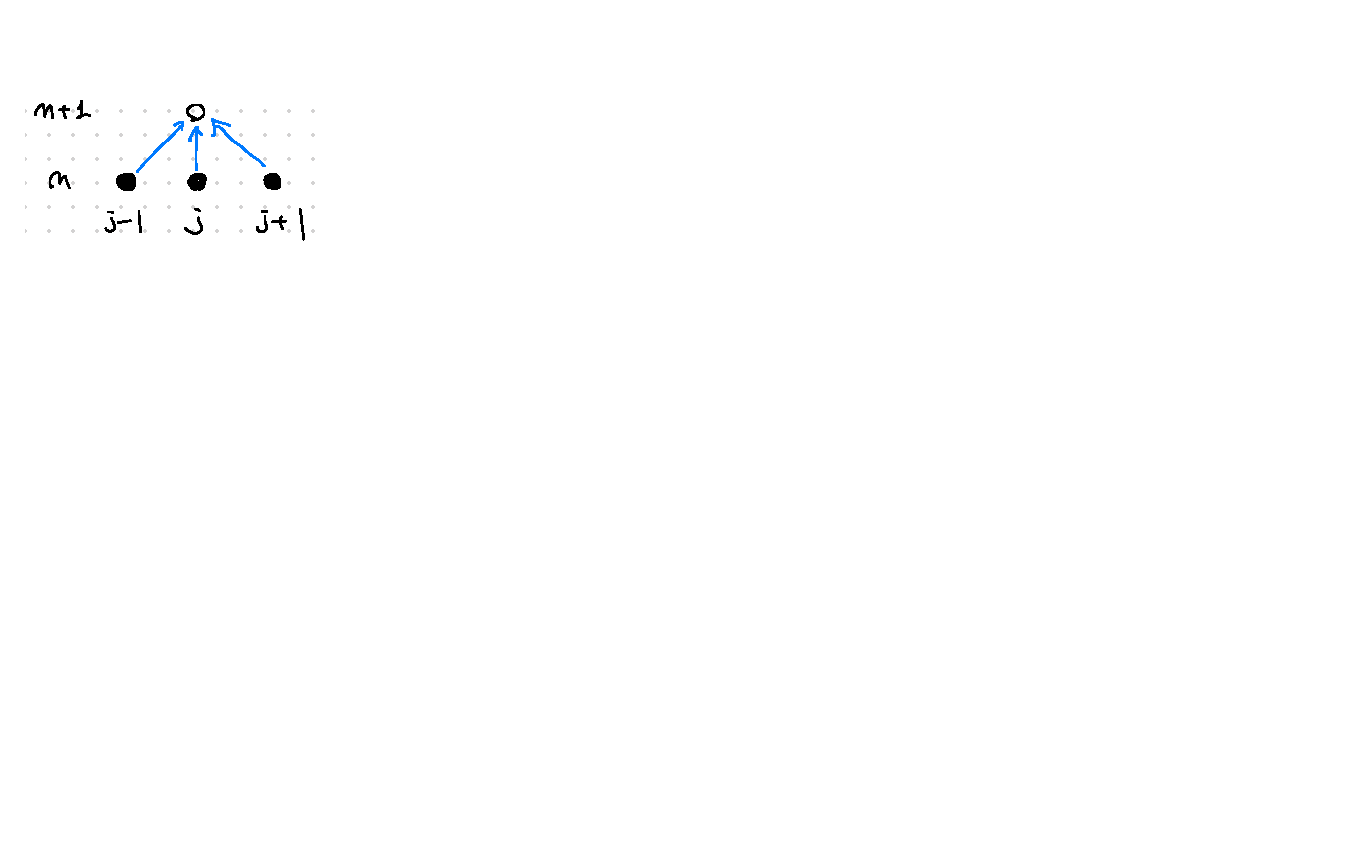
\includegraphics{image/ftcs-1.pdf}}
    \end{center}
  \item 初期条件
    \[
    u_j^0 = f(j\Delta x) \ \ (j=0,1,\cdots,N)
    \]
  \item 境界条件
    \[
    u_0^n = u_N^n = 0 \ \ (n=0,1,2,\cdots)
    \]
  \end{itemize}
\end{frame}

\begin{frame}[t]{有限差分法の安定性}
  \begin{itemize}
  \item (陽的)有限差分法においては、$\Delta t$、$\Delta x$は小さければ小さいほどよいというわけではない
  \item 一次元拡散方程式の場合
    \begin{align*}
      \begin{cases}
        r \le 1/2 & \text{安定} \\
        r > 1/2 & \text{\color{red}不安定}
      \end{cases}
    \end{align*}
  \item $\Delta x$を半分にしたら、$\Delta t$は1/4にしなければならない

    $\Rightarrow$ 計算量は8倍
  \end{itemize}
\end{frame}

\begin{frame}[t]{一次元波動方程式(双極型)}
  \begin{itemize}
  \item 一次元波動方程式
    \[
    \frac{\partial^2 u}{\partial t^2} = c^2 \frac{\partial^2 u}{\partial x^2} \qquad u(x,0)=f(x), \frac{\partial u}{\partial t} (x,0) = g(x)
    \]
  \item $t$に関する中心差分
    \[
    \frac{\partial^2 u}{\partial t^2} \Big|_{(j \Delta x, n \Delta t)} = \frac{u_{j}^{n+1} - 2 u_{j}^{n} + u_{j}^{n-1}}{\Delta t^2} + {\cal O}(\Delta t^2)
    \]
  \item 代入して整理すると
    \[
    u_{j}^{n+1} = 2u_{j}^{n} - u_{j}^{n-1} + \alpha^2 (u_{j+1}^{n} - 2 u_{j}^{n} + u_{j-1}^{n}) \qquad (\alpha = c\frac{\Delta t}{\Delta x})
    \]
  \end{itemize}
\end{frame}

\begin{frame}[t]{波動方程式に対するFTCS法}
  \begin{itemize}
  \item $O(\Delta t^2) + O(\Delta x^2)$の陽解法
    \begin{center}
      \resizebox{0.4\textwidth}{!}{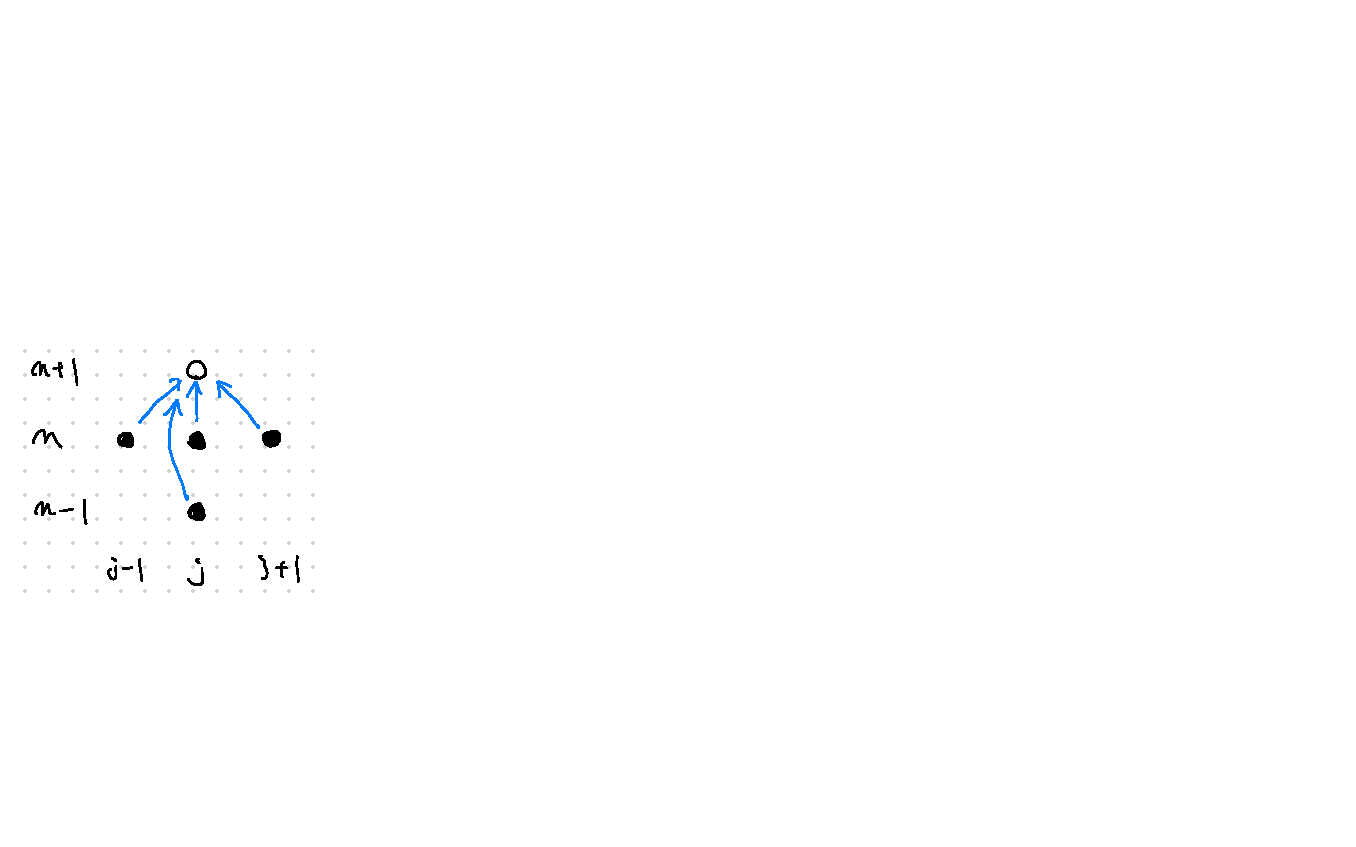
\includegraphics{image/ftcs-2.pdf}}
    \end{center}
  \item 初期条件
    \[
    u_j^0 = f(j\Delta x) \ \ (j=0,1,\cdots,N)
    \]
    初期速度については$n=0$に関する中心差分を考えて
    \[
    \frac{u_j^1 - u_j^{-1}}{2 \Delta t} = g_j \ \ \Rightarrow \ \ u_j^1 = u_j^0 + \Delta t g_j + \frac{\alpha^2}{2} (u_{j+1}^{n} - 2 u_{j}^{n} + u_{j-1}^{n})
    \]
  \end{itemize}
\end{frame}

\begin{frame}[t]{時間に依存するシュレディンガー方程式}
  \begin{itemize}
  \item 時間に依存するシュレディンガー方程式
    \[
    i \hbar \frac{\partial \Psi}{\partial t}(x,t) = H(x,t) \Psi(x,t) = \Big[ - \frac{\hbar^2}{2m} \frac{\partial^2}{\partial x^2} + V(x,t) \Big] \Psi(x,t)
    \]
    \begin{itemize}
    \item 波動関数のノルム $\displaystyle \int | \Psi(x,t) |^2 \, dx$ は保存
    \item $V(x,t)$が時間$t$に依存しない場合、エネルギーの期待値は保存
      \[
      \langle H \rangle = \frac{\displaystyle \int \Psi^* H \Psi \, dx}{\displaystyle \int | \Psi |^2 \, dx}
      \]
    \end{itemize}
  \item 以下では無次元化して$\hbar = m = 1$とおく
  \end{itemize}
\end{frame}

\begin{frame}[t]{時間に依存するシュレディンガー方程式}
  \begin{itemize}
  \item シュレディンガー方程式の形式解 ($V$が時間に依存しない場合)
    \[
    \Psi(x,t) = e^{-i H t} \Psi(x,0)
    \]
  \item $t$に関して前進差分
    \begin{align*}
      e^{-i H t} &= [e^{-i H \Delta t}]^M \approx [1 - i H \Delta t]^M \qquad (\Delta t = t / M) \\
      \Psi^{n+1} &= (1 -  i \Delta t H) \Psi^{n}
    \end{align*}
  \item $H$は対称(エルミート)行列 $\Rightarrow$ 時間発展演算子$e^{-i H \Delta t}$はユニタリー行列
  \item 差分近似$(1 -  i \Delta t H)$はユニタリーではない
    \begin{align*}
      & (e^{-i H \Delta t})^\dagger e^{-i H \Delta t} = e^{i H \Delta t} e^{-i H \Delta t} = 1 \\
      & (1 -  i \Delta t H)^\dagger (1 -  i \Delta t H) = (1 +  i \Delta t H) (1 -  i \Delta t H) = 1 + {\color{red} \Delta t^2 H^2}
    \end{align*}
  \end{itemize}
\end{frame}

\begin{frame}[t]{クランク・ニコルソン法}
  \begin{itemize}
  \item クランク・ニコルソン法
    \[
    \Psi^{n+1} = \frac{1 -  i \frac{\Delta t}{2} H}{1 +  i \frac{\Delta t}{2} H} \Psi^{n}
    \]
  \item (数値精度の範囲で)ユニタリー行列であるので、ノルムは保存
  \item $(1 +  i \frac{\Delta t}{2} H)^{-1}$を掛ける $\Rightarrow$ 連立一次方程式を解く必要がある
    \begin{itemize}
    \item まず、$\Psi = (1 - i \frac{\Delta t}{2} H) \Psi^n$ を計算
    \item 次に、$(1 +  i \frac{\Delta t}{2} H) \Psi^{n+1} = \Psi$ を解く(連立一次方程式)
    \end{itemize}
  \item 陰解法の一種
  \end{itemize}
\end{frame}

\begin{frame}[t]{拡散方程式に対する陰解法}
  \begin{itemize}
  \item 時刻$t$関して後退差分を使う
    \[
    \frac{\partial u}{\partial t} \Big|_{(j \Delta x, n \Delta t)} = \frac{u_j^{n} - u_j^{n-1}}{\Delta t} + {\cal O}(\Delta t)
    \]
  \item $x$に関する中心差分と組み合わせ、$n \rightarrow n+1$と書き直すと
    \[
    u_{j}^{n+1} = u_{j}^{n} + r (u_{j+1}^{n+1} - 2 u_{j}^{n+1} + u_{j-1}^{n+1})
    \]
    $u^{n+1}$が両辺に現れる $\Rightarrow$ 陰解法
  \item $O(\Delta t) + O(\Delta x^2)$
  \item $r$の値によらず{\color{red}常に安定}
  \end{itemize}
\end{frame}

\begin{frame}[t]{拡散方程式に対するクランク・ニコルソン法}
  \begin{itemize}
  \item さらに、時間方向にきざみ幅$\Delta t/2$の中心差分を使うと
    \[
    \frac{\partial u}{\partial t} \Big|_{(j \Delta x, n \Delta t)} = \frac{u_j^{n+\frac{1}{2}} - u_j^{n-\frac{1}{2}}}{\Delta t} + {\cal O}(\Delta t^2)
    \]
  \item $x$に関する中心差分と組み合わせ、$n \rightarrow n+\frac{1}{2}$し、さらに$u_j^{n+\frac{1}{2}}$を$(u_j^{n+1}+u_j^{n})/2$で近似すると
    \[
    u_{j}^{n+1} = u_{j}^{n} + \frac{r}{2} (u_{j+1}^{n+1} - 2 u_{j}^{n+1}  +u_{j-1}^{n+1} + u_{j+1}^{n} - 2 u_{j}^{n} + u_{j-1}^{n})
    \]
    あるいは
    \[
    u_{j}^{n+1} - \frac{r}{2} (u_{j+1}^{n+1} - 2 u_{j}^{n+1} + u_{j-1}^{n+1}) = u_{j}^{n} + \frac{r}{2} (u_{j+1}^{n} - 2 u_{j}^{n} + u_{j-1}^{n})
    \]
    $\Rightarrow$ クランク・ニコルソン法 [$O(\Delta t^2) + O(\Delta x^2)$]
  \end{itemize}
\end{frame}


\section{実習その3}

\begin{frame}[t,fragile]{EX3-1: サンプルプログラムの実行}
  \begin{itemize}
    %\setlength{\itemsep}{1em}
  \item[3-1-1] ガウスの消去法のサンプルプログラム(\href{https://github.com/todo-group/computer-experiments/blob/master/exercise/linear_system/gauss.c}{exercise/linear\_system/gauss.c})をコンパイル・実行せよ。実行時にコマンドライン引数に行列の内容が書かれたファイル名({\tt input1.dat})を指定する必要があることに注意
\begin{lstlisting}
$ cc gauss.c -o gauss
$ ./gauss input1.dat
\end{lstlisting}
  \item[3-1-2] LU分解のサンプルプログラム(\href{https://github.com/todo-group/computer-experiments/blob/master/exercise/linear_system/lu_decomp.c}{exercise/linear\_system/lu\_decomp.c})をコンパイル・実行せよ。コンパイル時にLAPACKをリンク({\tt -llapack})する必要があることに注意(ハンドブック3.1.6節)
\begin{lstlisting}
$ cc lu_decomp.c -o lu_decomp -llapack
$ ./lu_decomp input1.dat
\end{lstlisting}
  \end{itemize}
\end{frame}

\begin{frame}[t,fragile]{EX3-2: ピボット選択、境界条件}
  \begin{itemize}
    %\setlength{\itemsep}{1em}
  \item[3-2-1] {\tt gauss.c}では、ピボット選択を行っていないため、入力が{\tt input2.dat}の場合には正しい解が得られない。ピボット選択を行うよう{\tt gauss.c}を修正せよ
  \item[3-2-2] \href{https://github.com/todo-group/computer-experiments/blob/master/exercise/linear_system/laplace_lu.c}{exercise/linear\_system/laplace\_lu.c}では、ディリクレ型の境界条件[$u(0,y) = \sin(\pi y)$, $u(x,0)=u(x,1)=u(1,y)=0$]のもとでのラプラス方程式の解をLU分解により求めている。境界条件を変えてみて解がどのように変化するか、Gnuplotを用いてプロットして確認せよ(Gnuplotの{\tt splot}コマンドを使う)
  \end{itemize}
\end{frame}

\begin{frame}[t,fragile]{EX3-3: ヤコビ法、ガウス・ザイデル法、SOR法}
  \begin{itemize}
    %\setlength{\itemsep}{1em}
  \item[3-3-1] \href{https://github.com/todo-group/computer-experiments/exercise/blob/master/linear_system/laplace_jacobi.c}{exercise/linear\_system/laplace\_jacobi.c}は、作りかけのヤコビ法のプログラムである。収束判定のコードを追加し、プログラムを完成せよ。計算結果や計算速度を{\tt laplace\_lu.c}と比較せよ
  \item[3-3-2] ヤコビ法のプログラム({\tt lapalace\_jacobi.c})を元に、ガウス・ザイデル法、SOR法のプログラムを作成せよ。収束までの回数を比較せよ。
特にSOR法の場合、パラメータ$\omega$の選び方により、どのように収束回数が変化するか観察し、最適な$\omega$の値について考察せよ
  \end{itemize}
\end{frame}


\end{document}
